
\section{Cycle-Consistent Adversarial Domain Adaption}

\begin{figure}
  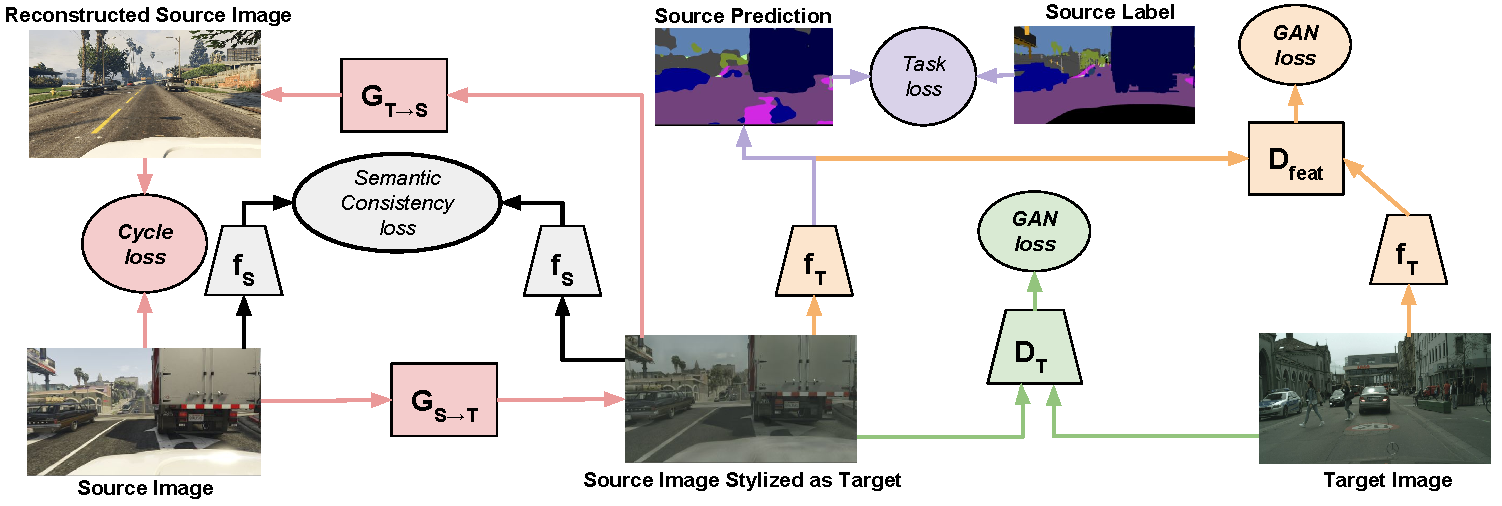
\includegraphics[width=\textwidth]{figs/cycada_method_src_colored.pdf}
  \caption{
    Cycle-consistent adversarial adaptation of pixel-space inputs.
    %We train our model in two stages.
    By directly remapping source training data into the target domain, we remove the low-level differences between the domains, ensuring that our task model is well-conditioned on target data. We depict here the image-level GAN loss (\textcolor{green}{green}), the feature level GAN loss (\textcolor{orange}{orange}), the source and target semantic consistency losses (black), the source cycle loss (\textcolor{red}{red}), and the source task loss (\textcolor{purple}{purple}). For clarity the target cycle is omitted. 
  }
  \label{fig:implementation}
\end{figure}

We consider the problem of unsupervised adaptation, where we are provided source data $X_S$, source labels $Y_S$, and target data $X_T$, but no target labels.
The goal is to learn a model $f$ that can correctly predict the label for the target data $X_T$.

We can begin by simply learning a source model $f_S$ that can perform the task on the source data.
For $K$-way classification with a cross-entropy loss, this corresponds to
%%%%%%%%%%%% L_Task %%%%%%%%%%%%
\begin{align}
  \loss_{\text{task}}(f_S, X_S, Y_S) = 
  		- \mathbb{E}_{\small{(x_s, y_s) \sim (X_S, Y_S)} }
        \sum_{k=1}^K \mathbbm{1}_{[k = y_s]} \log \left( \sigma(f_S^{(k)}(x_s)) \right) 
\end{align}
%%%%%%%%%%%%%%%%%%%%%%%%%%%%%%%%
where $\sigma$ denotes the softmax function. 
However, while the learned model $f_S$ will perform well on the source data, typically domain shift between the source and target domain leads to reduced performance when evaluating on target data.
To mitigate the effects of domain shift, we follow previous adversarial adaptation approaches and learn to map samples across domains such that an adversarial discriminator is unable to distinguish the domains.
By mapping samples into a common space, we enable our model to learn on source data while still generalizing to target data.

To this end, we introduce a mapping from source to target $\StoT$ and train it to produce target samples that fool an adversarial discriminator $D_T$.
Conversely, the adversarial discriminator attempts to classify the real target data from the source target data.
This corresponds to the loss function
%%%%%%%  L_GAN %%%%%%%%%%
\begin{align}
  \label{eq:gan-loss}
  \lossgan( G_{S \rightarrow T}, D_T, X_T, X_S) = \mathbb{E}_{x_t \sim X_T}\left[\log D_T(x_t)\right]
    + \mathbb{E}_{x_s \sim X_S}\left[\log(1 - D_T(\StoT(x_s)))\right] 
\end{align}
%%%%%%%%%%%%%%%%%%%%%%%%
This objective ensures that $\StoT$, given source samples, produces convincing target samples.
In turn, this ability to directly map samples between domains allows us to learn a target model $f_T$ by minimizing $\loss_{\text{task}}(f_T, \StoT(X_S), Y_S)$ (see Figure~\ref{fig:implementation} green portion).


However, while previous approaches that optimized similar objectives have shown effective results, in practice they can often be unstable and prone to failure.
Although the GAN loss in Equation~\ref{eq:gan-loss} ensures that $\StoT(x_s)$ for some $x_s$ will resemble data drawn from $X_T$, there is no way to guarantee that $\StoT(x_s)$ preserves the structure  or content of the original sample $x_s$.

In order to encourage the source content to be preserved during the conversion process, we impose a cycle-consistency constraint on our adaptation method~\citep{zhu_arxiv17,yi2017dualgan,kim_arxiv17} (see Figure~\ref{fig:implementation} red portion).
To this end, we introduce another mapping from target to source $\TtoS$ and train it according to the same GAN loss $\lossgan(\TtoS, D_S, X_S, X_T)$.
We then require that mapping a source sample from source to target and back to the source reproduces the original sample, thereby enforcing cycle-consistency.
In other words, we want $\TtoS(\StoT(x_s)) \approx x_s$ and $\StoT(\TtoS(x_t)) \approx x_t$.
This is done by imposing an L1 penalty on the reconstruction error, which is referred to as the \emph{cycle-consistency loss}:
%%%%%% L_cyc  %%%%%%%%%%%%
\begin{align}
  \label{eq:cycle-loss}
  \mathcal{L}_\text{cyc}(\StoT,  \TtoS, X_S, X_T) &=
   \mathbb{E}_{x_s \sim X_S}\left[||\TtoS(\StoT(x_s)) - x_s||_1\right] \\
  &+  \mathbb{E}_{x_t \sim X_T}\left[||\StoT(\TtoS(x_t)) - x_t||_1\right].\nonumber
\end{align}
%%%%%%%%%%%%%%%%%%%%%%%%%%
%
Additionally, as we have access to source labeled data, we explicitly encourage high semantic consistency before and after image translation. %We train a source task model, , and 
We pretrain a source task model $f_S$, fixing the weights, we use this model as a noisy labeler by which we encourage an image to be classified in the same way after translation as it was before translation according to this classifier. Let us define the predicted label from a fixed classifier, $f$, for a given input $X$ as $p(f,X) = \text{arg} \max(f(X))$. Then we can define the semantic consistency before and after image translation as follows:
%%%%%% L_sem  %%%%%%%%%%%
\begin{align}
	\label{eq:semantic}
	\mathcal{L}_\text{sem}(\StoT, \TtoS, X_S, X_T, f_S) &=
	 \mathcal{L}_{\text{task}}(f_S, \TtoS(X_T), p(f_S, X_T))  \\
	&+  \mathcal{L}_{\text{task}}(f_S, \StoT(X_S), p(f_S, X_S)) \nonumber 
\end{align}
%%%%%%%%%%%%%%%%%%%%%%%%%%
See Figure~\ref{fig:implementation} black portion. This can be viewed as analogously to content losses in style transfer ~\citep{gatys2016image} or in pixel adaptation \citep{dtn}, where the shared content to preserve is dictated by the source task model $f_S$.

We have thus far described an adaptation method which combines cycle consistency, semantic consistency, and adversarial objectives to produce a final target model. As a pixel-level method, the adversarial objective consists of a discriminator which distinguishes between two image sets, e.g. transformed source and real target image. Note that we could also consider a feature-level method which discriminates between the features or semantics from two image sets as viewed under a task network. This would amount to an additional feature level GAN loss (see Figure~\ref{fig:implementation} orange portion):
\begin{equation}
	\lossgan(f_T, D_\text{feat}, f_S(\StoT(X_S)), X_T).\label{eq:adversarial-feature}
\end{equation}


Taken together, these loss functions form our complete objective:
%%%%%% L_cycada  %%%%%%%%%%%%
\begin{align}
  \label{eq:cycada}
  \loss_{\text{CyCADA}}&(f_T, X_S, X_T, Y_S, \StoT, \TtoS, D_S, D_T) \\
  &= \loss_{\text{task}}(f_T, \StoT(X_S), Y_S) \nonumber \\
  &+ \lossgan(\StoT, D_T, X_T, X_S)
  + \lossgan(\TtoS, D_S, X_S, X_T) \nonumber \\
  &+ \lossgan(f_T, D_\text{feat}, f_S(\StoT(X_S)), X_T)\nonumber \\
  &+ \loss_\text{cyc}(\StoT, \TtoS, X_S, X_T)
  + \mathcal{L}_\text{sem}(\StoT, \TtoS, X_S, X_T, f_S). \nonumber
\end{align}
%%%%%%%%%%%%%%%%%%%%%%%%%%%%%

This ultimately corresponds to solving for a target model $f_T$ according to the optimization problem
%%%% f* %%%%%
\begin{equation}
   f_T^* = \argmin_{f_T} \min_{\substack{\StoT\\ \TtoS}} \max_{D_S, D_T} \loss_\text{CyCADA}(\small{f_T, X_S, X_T, Y_S, \StoT, \TtoS, D_S, D_T}).
\end{equation}
%%%%%%%%%%%%%%

We have introduced a method for unsupervised adaptation which generalizes adversarial objectives to be viewed as operating at the pixel or feature level. In addition, we introduce the use of cycle-consistency together with semantic transformation constraints to guide the mapping from one domain to another. 
In this work, we apply CyCADA to both digit adaptation and to semantic segmentation. We implement $G$ as a pixel-to-pixel convnet, $f$ as a convnet classifier or a Fully-Convolutional Net (FCN) and $D$ as a convnet with binary outputs.
